\section{Aufbau der Einzelbauteile}
Die zweidimensionalen Strukturen der DCEL werden genutzt, um das 3D-Model, welches aus SCAD-Objekten besteht, zu erstellen.
Dabei werden Modifikationen an allen Bauteilen vorgenommen, folgende Kriterien erfüllt sind:\\
Das 3D-Modell soll...
\begin{compactenum}
	\item ...einfach aufgebaut werden können.
	\item ...einen angemessenen Einblick in die Immobilie gewährleisten.
	\item ...stabil sein, auch nachdem einzelne Elemente entfernt wurden.
\end{compactenum}
Für die Erfüllung dieser Kriterien wurden die drei Strukturen Wand, Eckpfeiler und Grundplatte entworfen.
Weiterführend sind diese so modifiziert, dass sie ein oben beschriebenes 3D-Konstrukt darstellen.

\subsection{Eckpfeiler}
Die Eckpfeiler des Modells symbolisieren die Knoten Grundrisses.
Sie sind das Schlüsselelement des implementierten Stecksystems, welches für Stabilität und Variabilität sorgt.
Damit anliegende Wände und Grundplatten in einen Eckpfeiler greifen können, sind zwei verschiedene Arten von Steckern entworfen wurden.
Diese sind an zwei voneinander unabhängigen Abschnitten \q{CornerPin} und \q{CornerCylinder} angebracht, welche zusammengefügt das gesamte 3D-Objekt verkörpern.
\begin{Bild}{Ein Eckpfeiler (Screenshot der Verfasser)}
	
\includegraphics[height=200px]{Bilder/Untereinheit_Ecke}
\end{Bild}
\subsubsection{CornerCylinder}
Der \q{CornerCylinder} stellt den oberen Teil des Eckpfeilers dar.
Dieser besteht aus einem zylindrischen Grundbauteil mit Vertiefungen.
Diese Entstehen, indem Schnittmengen zwischen dem Zylinder und in Richtung der ausgehenden Kanten gedrehten Quader gebildet werden.
Nun können Wände in diese eingeschoben werden.
\begin{Bild}{Querschnitt eines CornerCylinders mit zwei angrenzenden Wänden}
	
\includegraphics[height=150px]{Bilder/CornerCylinder2D-06.png}
\end{Bild}

%\todoinline{Abbildungen?}
\subsubsection{CornerPin}
Die Summe aller Objekte des Typs \q{CornerPin} repräsentieren den untere Abschnitt des Eckpfeilers, welcher die Verbindungen der Grundplatten mit diesem gewährleistet.
Hierfür besteht ein einzelner \q{CornerPin} aus einem Zylinder, einer Ausstülpung seitens diesem und einem Zylindersegment.
Der Zylinder wird durch den Basiszylinder des Eckpfeilers festgelegt, welcher auch beim \q{CornerCylinder} vorkommt.
Für die Ausstülpung gilt, dass sie aus einem Quader mit einem angrenzendem Zylinder aufgebaut ist.
Die Länge des Quaders ist dabei abhängig von dem Winkel zwischen den beiden Wänden, welche die Grundplatte an dem Eckpfeiler begrenzen.
Er wird stets so lang berechnet, dass die Ausstülpung(siehe Abbildung, grün dargestellt) einen definierten Abstand von den Wänden einnimmt(siehe \ref{params}).
Für die untere Abgrenzung des Pinkopfes(siehe Abbildung, hellblau) berechnet die Anwendung eine Schnittmenge zwischen der angrenzenden Fläche und einem flachen Zylinder.\\
Falls ein \q{CornerPin} für das äußere Gebiet berechnet werden soll, wird anstatt der oben beschriebenen Elementen eine Differenzmenge zwischen der Umrandungsfläche des Grundisses und dem flachen Zylinder gebildet.
Dies resultiert in ein Zylindersegment, wie es in \todo{Wie referenziert man auf Abbildungen?}(rot) zu sehen ist.
Ein Eckpfeiler hat so einen stabilisierten unteren Abschnitt, auch wenn er außen im Grundriss liegt.

\begin{Bild}{Draufsicht auf den unteren Abschnitt eines Eckpfeilers}
	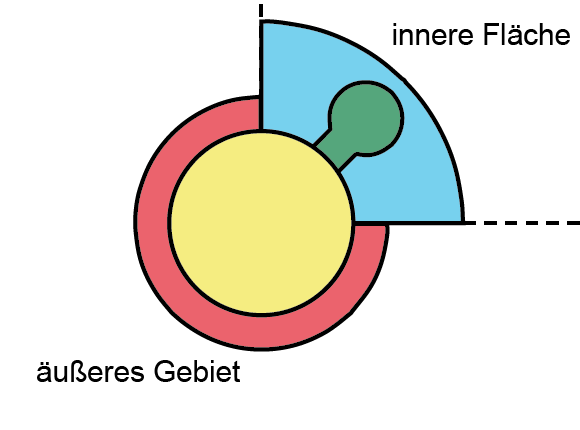
\includegraphics[height=150px]{Bilder/CornerPin2D-07.png}
\end{Bild}
\subsection{Wandstücke}
Die Wände des Modells verkörpern die Kanten des Grundrisses.

\begin{Bild}{Querschnitt einer Wand}
	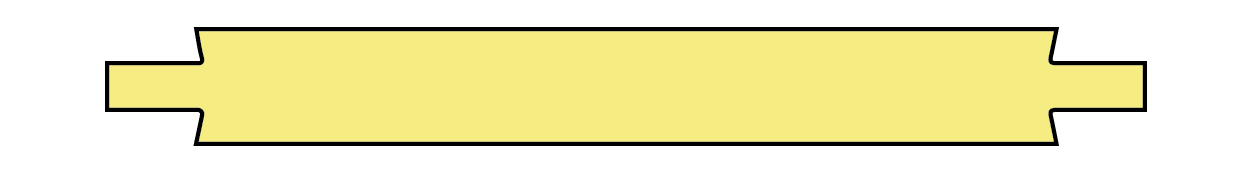
\includegraphics[width = 100mm]{Bilder/Wand2D-04}
\end{Bild}
\begin{Bild}{Ein Wandteil (Screenshot der Verfasser)}
	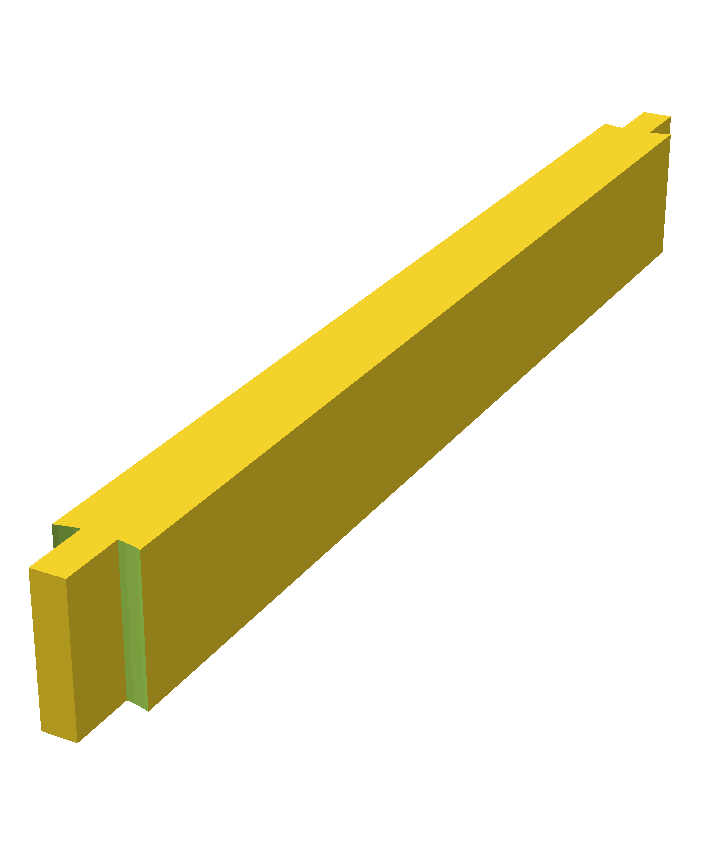
\includegraphics[height=200px, width=240px]{Bilder/Untereinheit_Wand}
\end{Bild}
Der größte dieser Quader stellt, wie in Abbildung~\thebildnr\ zu sehen, den mittleren Hauptteil dar.
Dieser Teil verfügt über die tatsächliche Länge der Wand, welche im Grundriss angegeben ist.
Die Höhe und Breite der Wand werden jedoch mit konstanten Parametern zu Beginn des Programmes festgelegt. \\
%Einer dieser Quader stellt das mittlere Wandstück dar, welches die wirkliche Wand repräsentiert und somit die entsprechende Länge und die definierte \icode{WallWidth} Wandbreite besitzt.
Die zwei kleineren Quader dienen dem Befestigen der Wand am Eckpfeiler.
Dafür wurden die beiden Quader mittig an die beiden schmalen Seiten des Mittelteils gesetzt.
Die Verbindungsstücke verfügen dabei über die gleiche Höhe wie die eigentliche Wand, ihre Breite beträgt aber nur ein Drittel der Wandbreite.\\
\todoinline{Details über die Länge der Pins hinzufügen!}
%Zwei kleinere werden eingesetzt um die Verankerung mit den Eckpfeilern zu garantieren.
%Diese werden am Anfang und Ende des Mittelstückes angelegt und können so an den Enden in die Eckzylinder greifen.
\todoinline{$\varepsilon$?}



\subsection{Grundplatten}
Grundplatten repräsentieren die Flächen des Grundrisses.
Sie sind aufgebaut aus einem extrudierten Polygon, welches inverse Steckmechanismen am Boden aufweist.
\begin{Bild}{Eine Grundplatte (Screenshot der Verfasser)}
	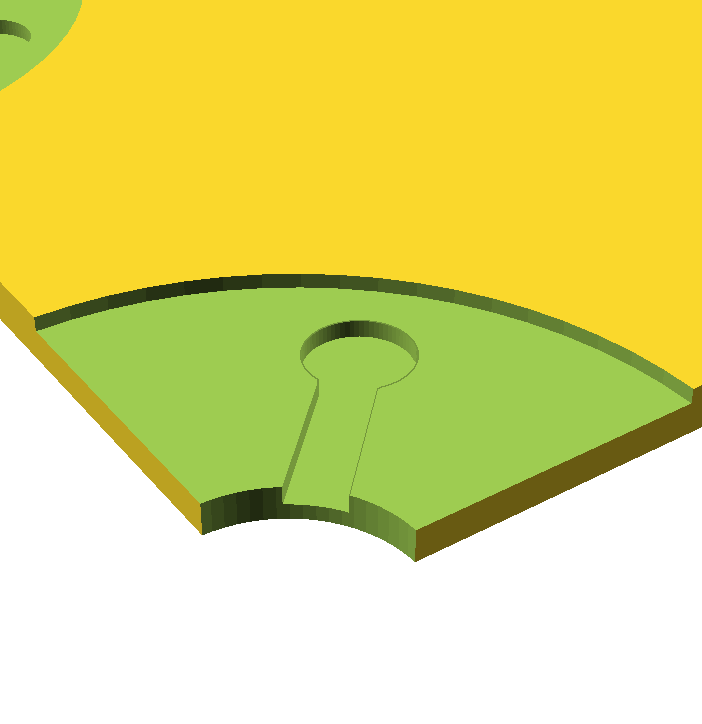
\includegraphics[height=200px]{Bilder/Untereinheit_GP}
\end{Bild}
Ein Ausschnitt einer solchen Grundplatte ist in Abbildung~\thebildnr\ zu sehen.
Die inversen Steckmechanismen dienen dem Anbringen der Grundplatte an die Eckpfeiler.
Für jeden Knoten, der an der Fläche anliegt wird hierbei je eine Einkerbung vorgenommen, die auf das Stecksystem des zu dem Knoten zugehörigen Eckpfeiler passt.
%Diese werden durch Differenzen des Ausgangspolygon mit dem negativen komplementären CornerPin realisiert.
%So entsteht für jeden Knoten der Fläche eine Einkerbung für die Verankerung.
\todoinline{Abstand zwischen Flächen; Vergrößerung von an das äußere Gebiet angrenzende Fläche}

\subsection{Zuweisen von Berechnungskonstanten}
\label{params}
\subsubsection{Funktion der \icode{Params}-Klasse}
Die \icode{Params}-Klasse wird als statische Zugriffsmöglichkeit auf bestimmte Konstanten des Programms verwendet, welche bei der Berechnung der Bauteile vonnöten sind.
Diese Klasse verfügt hierbei über öffentliche statische Funktionen, mit der aus allen anderen Klassen ohne eine Instanziierung der \icode{Params}-Klasse deren Parameter gesetzt oder auf bereits vorhandene Parameter zugegriffen werden kann.
Die Statik der Variablen und Funktionen verhindert hierbei, dass während des Programmablaufes verschiedene  Berechnungskomponenten unterschiedliche Konstanten zur Verfügung gestellt bekommen. \\
Das Setzen der Parameter findet zu Beginn des Programmes in der \icode{Main}-Klasse statt.
Hierbei wird die Funktion \icode{setParams()} aufgerufen.
Dieser Funktion werden sämtliche Werte als Parameter des Datentyps \icode{double} übergeben.
In der \icode{Params}-Klasse werden dann innerhalb der Funktion allen privaten Variablen ihre Werte entsprechend der Parameter zugewiesen und abrufbar gemacht.\\

\begin{code} [Die \icode{setParams()}-Funktion zum Setzen der Parameter]
	public static void setParams(double E, ...){
		e = E;
		// ...
	}
\end{code}

Das Abrufen der Parameter erfolgt dann mittels der entsprechenden \icode{get()}-Funktionen der \icode{Params}-Klasse, welche für alle Parameter vorhanden sind.
Ein Überschreiben einzelner Parameter wird an dieser Stelle verhindert, da für die privaten Variablen keine \icode{set()}-Funktionen vorliegen.
Der Aufbau der \icode{get()}-Funktionen folgt dem generellen Aufbau des nachfolgenden Codebeispiels, jedoch werden die Parameterbezeichnungen jeweils entsprechend ersetzt:\\

\begin{code} [Die \icode{get()}-Funktion für den Parameter \icode{e}]
public static double getE() {
	return e;
}
\end{code}

Diese Funktionen werden dann aus den Programmteilen, in denen sie für Berechnungen benötigt werden, statisch mittels des Aufrufs der \icode{Params}-Klasse aufgerufen. \\
Die Bedeutung der einzelnen Parameter erklärt sich wie folgt:

\begin{description}[style=nextline]
	\item[E ($\epsilon$/Epsilon)] 
		Der Parameter \q{E} entspricht der Konstante $\epsilon$ (Epsilon), welcher aus Gründen der vorteilhaften Kürze der Parameternamen hier verwendet wurde.
		Somit muss nicht jedes mal \icode{Epsilon} ausgeschrieben werden, es wird auf \icode{E} reduziert.
		$\epsilon$ bezeichnet den Abstand, welcher zwischen zwei Bauteilen mit einberechnet werden muss, um ein einfaches Zusammenstecken zu gewährleisten.
	\item[CornerRadius]
		Der Parameter \q{CornerRadius} entspricht der Konstante, welche den Radius des Grundzylinders der Eckstücken angibt.
	\item[PinMinLength] 
		Der Parameter \q{PinMinLength} entspricht der Konstante, welche die minimale Länge des Quaders des positiven Eckstücks angibt, welcher zwischen dem Eckzylinder und dem Pinzylinder platziert wird.
	\item[PinPWidth] 
		Der Parameter \q{PinPWidth} entspricht der Konstante, welche die Weite für den Quader des positiven Eckstücks angibt, welcher zwischen dem Eckzylinder und dem Pinzylinder platziert wird.
	\item[PinPRadius] 
		Der Parameter \q{PinPRadius} entspricht der Konstante, welche den Radius des Pinzylinders des positiven Eckstücks angibt.
	\item[PinDistance]
		Der Parameter \q{PinDistance} entspricht der Konstante, welche die Distanz zwischen dem positiven Pin und den anliegenden Wandstücken angibt, welche für jeden Pin eingehalten werden muss.
	\item[Height]
		Der Parameter \q{Height} entspricht der Konstante, welche die Höhe der Wandteile und der Eckzylinder angibt.
	\item[PinHeight]
		Der Parameter \q{PinHeight} entspricht der Konstante, welche die Höhe des positiven Pinzylinders angibt.
	\item[BasePlateHeight]
		Der Parameter \q{BasePlateHeight} entspricht der Konstante, welche die Höhe der Grundplatte angibt.
	\item[BasePlatePinCircleHeight]
		Der Parameter \q{BasePlateCircleHeight} entspricht der Konstante, welche die Höhe der Kreisflächen angibt, die unter den positiven Eckstücken angebracht werden und der Stabilisierung und Verankerung von Grundplatter und Eckstück dienen.
\end{description}